\documentclass[12pt]{article}
\usepackage[english]{babel}
\usepackage[utf8x]{inputenc}
\usepackage[T1]{fontenc}
\usepackage{scribe}
\usepackage{listings}
\usepackage{enumitem}

\Scribe{}
\Lecturer{Abir De}
\LectureNumber{18}
\LectureDate{16 October, 2022}
\LectureTitle{Tutorial 2 (Gaussian Processes)}

\lstset{style=mystyle}

\begin{document}
	\MakeScribeTop

\noindent In this tutorial, we explore the theory behind Gaussian Processes, and solve a few problems based on them.

\section{Basics of Bayesian Theory}
% Sarthak

Consider a Binomial Random Variable (i.e. an experiment involving repeated $N$ Bernoulli trials) that denotes toss of a coin repeated $N$ times. We report an estimate for the bias of the coin $p$ as $\hat{p} = \mathbb{E}\left[\# \text{heads}\right]$. This is referred to as Maximum Likelihood Estimate. When $N$ is small, this estimate is very poor and thus we see Bayesian theory that gives us reasonable estimates in low data regimes.

\subsection{Prior}
% Sarthak

The concept of a prior distribution is that it gives us some additional information, or in a way, it is our initial belief, about the parameters involved in the distribution. For example, for the above mentioned problem, we would choose the prior to be a \textbf{Beta distribution} with parameters $\alpha$ and $\beta$ chosen such that $\alpha = \beta = c$, where $c$ is some constant, such that the mean of the prior distribution is $\displaystyle \frac{1}{2}$, and variance is some suitable fraction.

\subsection{Likelihood}
% Sarthak

The likelihood tells us more about the data and the probability associated with the input instance, given the parameters (conditional probability). We wish to use the data to find (or more precisely, \textbf{estimate}) the parameters that better fit the data. To estimate the parameters, we use \textbf{Baye's rule} of conditional probability.

\subsection{Estimation}
% Sarthak

We compute the posterior distribution by taking the product of the prior distribution with the likelihood, thus computing the conditional probability of parameters given the data. Mathematically: \[ P(\theta|D) = \frac{P(D|\theta) \cdot P(\theta)}{P(D)} \]
Here, $\theta$ represents the set of parameters. The LHS represents the \textbf{posterior}, the RHS numerator represents product of \textbf{likelihood} and \textbf{prior}, and the RHS denominator, which is primarily for normalisation (so that the distribution integrates to 1), represents the \textbf{marginal} on the data, which is essentially $\displaystyle \sum_{\theta} P(D|\theta) \cdot P(\theta)$. We then determine the estimate using the posterior distribution (maximum value estimation).

\subsection{Degeneracy}
% Sarthak

If we have not seen much data, the estimate essentially falls back to the prior distribution. On the other hand, if there is lot of data, the posterior estimate tends to the data, and prior effectively is ignored. These degenerate cases also occur if there is extreme precision (variance tends to 0) or unreliability (variance is large) in the prior, because the estimate that we find varies roughly in the form: \[ \mu_{MAP} = \frac{N \mu_D \sigma_P ^ 2 + \mu_P \sigma_D ^ 2}{N \sigma_P ^ 2 + \sigma_D ^ 2} \]
Consider the cases when $N \rightarrow 0$, $N \rightarrow \infty$, $\sigma_P \rightarrow 0$ and $\sigma_P \rightarrow \infty$.

\section{Gaussian \& Multi-variate Gaussian}
% Sarthak

Analogous to the one-dimensional Gaussian distribution denoted by $X \sim \mathcal{N}(\cdot | \mu, \sigma)$, we have the multi-variate Gaussian distribution $X \in \R^n \sim \mathcal{N}(\cdot | \vec{\mu}, \Sigma^{n \times n})$, where $\Sigma^{n \times n}$ is the covariance matrix defined as $\Sigma(i,j) = cov(X_i,X_j)$. For parametrizing an MVG distribution, we use $m(X)$ as the estimate for $\mu$ and $K(x,x')$ as the estimate for $\Sigma$ where the kernel function $K(\cdot,\cdot)$ is chosen keeping properties of the covariance matrix in mind (symmetric and positive semi-definite).

\section{Gaussian Processes}
% Sarthak

We introduce the problem statement for fitting a Gaussian Process to a dataset. Given the training data $\displaystyle D = {(\mathbf{x}_i,y_i)}_{i = 1}^N$, we make a few basic assumptions:

\begin{itemize}
    \item $y = f(x) + \epsilon; \epsilon \sim \mathcal{N}(0,\sigma_\epsilon^2)$
    \item Prior [$f(\mathbf{x}_i), \dots, f(\mathbf{x}_N)$] $\sim \mathcal{N}(0,K)$
    \item Target [$y_1, \dots, y_N | \mathbf{f}$] $\sim \mathcal{N}(\mathbf{f},\sigma^2)$
\end{itemize}

\noindent Theoretically, we consider that $\epsilon$ is \textbf{irreducible noise} that we do not model (not in our control). We assume a prior on the relation between $x$ and $y$. The task, which is sampling values of the function $f$, reduces to conditional probability involving the data. The problem is thus essentially: \\

\noindent \textbf{Question.} For a test point $\mathbf{x}^*$, find the label $y^*$. Since noise is zero-mean, we will proceed to find $P(f^*|\mathbf{x}^*,D)$. The labels $y^*$ will then follow $\mathcal{N}(\cdot | f^*, \sigma_\epsilon)$.

\section{Determining $P(f^*|\mathbf{x}^*,D)$}
% Sarthak

To find the distribution $P(f^*|\mathbf{x}^*,D)$, we introduce $f$ and then use Baye's rule:

\vspace{-1em}

\begin{align*}
    P(f^*|\mathbf{x}^*,D) &= \int_{f_1, \dots, f_N} P(f^*,f_1,\dots,f_N|\mathbf{x}^*,D) d\mathbf{f} \\
    &= \int_{\mathbf{f}} P(f^*|\mathbf{f},\mathbf{x}^*,D) \cdot P(\mathbf{f}|\mathbf{x}^*,D) d\mathbf{f}
\end{align*}

\subsection{Data Likelihood $P(\mathbf{f}|\mathbf{x}^*,D)$}
% Sarthak

\textbf{Question.} Can you remove some terms from the conditioning set? \\
\noindent \textbf{Ans:\hspace{3mm}} Analysing the expression, we can conclude that for the function $f$, given the data $D$, $x^*$ is not relevant. For determining $P(\mathbf{f}|D)$, we need $P(D|\mathbf{f})$ and then using the prior $P(\mathbf{f})$, we can find the data likelihood using Baye's rule. We have, $P(D|\mathbf{f}) = P(\{(x_i,y_i)\} | \mathbf{f})$. \\

\noindent \textbf{Question.} Simplify this further and obtain an expression for the data likelihood. Note that the expression should not involve $\mathbf{x}$. \\
\noindent \textbf{Ans:\hspace{3mm}} Since we are under supervised setting, $\mathbf{x}$ is fixed and so can be moved over to conditions. Now given $\mathbf{f}$, $y$ does not depend on $\mathbf{x}$.

\vspace{-1em}

\begin{align*}
    P(D|\mathbf{f}) &= P(\{(x_i,y_i)\} | \mathbf{f}) \\
    &= P(\{y_i\} | \{x_i\}, \mathbf{f}) \\
    &= P(\{y_i\} | \mathbf{f})
\end{align*}

\noindent By analytically evaluating, we get the data likelihood as: \[ P(\mathbf{f}|D) = \mathcal{N}(K(K + \sigma^2 I)^{-1} \mathbf{y}, \sigma^2 K(K + \sigma^2 I)^{-1}) \]

\noindent \textbf{Question.} When will the data likelihood be maximum? When will the GP perfectly fit the dataset? \\
\noindent \textbf{Ans:\hspace{3mm}} When the standard deviation is high, the data does not fit at all and the estimate falls back to the prior. On the other hand, when $\sigma \rightarrow 0$, we trust the data to the fullest, $K$ is invertible and so the data fits perfectly.

\subsection{Joint Distribution $P(\mathbf{f},f^*)$}
% Sarthak

Define $\mathbf{k} \equiv [\mathcal{K}(\mathbf{x}^*,\mathbf{x}_1),\dots,\mathcal{K}(\mathbf{x}^*,\mathbf{x}_N)]^T$. Then the joint distribution of $[\mathbf{f} \text{ } f^*]^T$ is: \[ \begin{bmatrix}
    \mathbf{f} \\
    f^*
\end{bmatrix} \sim \mathcal{N} \left( \mathbf{0}, \begin{bmatrix}
    K & \mathbf{k} \\
    \mathbf{k}^T & \mathcal{K}(\mathbf{x}^*,\mathbf{x}^*)
\end{bmatrix} \right) \]

\subsection{Marginal and Conditional}
% Sarthak

For multi-variate Gaussian Processes, we can determine the marginal and conditional distribution using the joint distribution using the following properties: \[ P_{X,Y} \sim \mathcal{N}(\mu,\Sigma) = \mathcal{N} \left( \begin{bmatrix}
    \mu_X \\
    \mu_Y
\end{bmatrix}, \begin{bmatrix}
    \Sigma_{XX} & \Sigma_{XY} \\
    \Sigma_{YX} & \Sigma_{YY}
\end{bmatrix} \right) \]

\noindent We have $X \sim \mathcal{N}(\mu_X,\Sigma_{XX})$ and $Y \sim \mathcal{N}(\mu_Y,\Sigma_{YY})$ then: \[ X | Y \sim \mathcal{N}(\mu_X + \Sigma_{XY} \Sigma^{-1}_{YY} (Y - \mu_Y), \Sigma_{XX} - \Sigma_{XY} \Sigma^{-1}_{YY} \Sigma_{YX}) \] \[ Y | X \sim \mathcal{N}(\mu_Y + \Sigma_{YX} \Sigma^{-1}_{XX} (X - \mu_X), \Sigma_{YY} - \Sigma_{YX} \Sigma^{-1}_{XX} \Sigma_{XY}) \]

\noindent Using these, we can find out the marginal $P(f^*)$ and conditional $P(f^*|\mathbf{f})$ distributions. Coming back to the integral:

\[ P(f^*|\mathbf{x}^*,D) = \int_{\mathbf{f}} P(f^*|\mathbf{f},\mathbf{x}^*,D) \cdot P(\mathbf{f}|\mathbf{x}^*,D) d\mathbf{f} \]

\noindent \textbf{Question.} Why is the result of the above integration Gaussian? \\
\noindent \textbf{Ans:\hspace{3mm}} Since both would be Gaussian, and the data likelihood is also a Gaussian, the resulting distribution for $P(f^*|\mathbf{x}^*,D)$ after integration will also be a Gaussian. Solving the integration gives us: \[ P(f^*|\mathbf{x}^*,D) = \mathcal{N} \left( \mathbf{k}^T (K + \sigma^2 I)^{-1} \mathbf{y}, \mathcal{K}(\mathbf{x}^*, \mathbf{x}^*) - \mathbf{k}^T (K + \sigma^2 I)^{-1} \mathbf{k} \right) \]

\vspace{1em}

\noindent \textbf{Question.} Do the labels $\mathbf{y}$ affect the variance of $f^*$?\\
% Annam 
\noindent \textbf{Ans:\hspace{3mm}} We can see that variance \( = \mathcal{K}(\mathbf{x}^*, \mathbf{x}^*) - \mathbf{k}^T (K + \sigma^2 I)^{-1} \mathbf{k} \)\\
As you can see, the variance of posterior distribution does not have any term related to labels, we can safely say that answer is No.

\subsection{1-Nearest Neighbor Regressor}
% Sarthak

\textbf{Question.} How should $\mathbf{k}$ look like for the above equation to act as a 1-nearest neighbor regressor? \\
\noindent \textbf{Ans:\hspace{3mm}} Suggestion from a student: we can use the Euclidean distance function $d(\mathbf{x}_i,\mathbf{x}_j)$. We then add a threshold $\mathbf{\beta}$ defined as $\beta_i = d(\mathbf{x}^*,\mathbf{x}_i) + \epsilon_i$. We can then define the kernel function as: \[ k(\mathbf{x}_i,\mathbf{x}_j) = \begin{cases}
    1 & d(\mathbf{x}_i,\mathbf{x}_j) < \beta_j \\
    0 & otherwise
\end{cases} \]

\noindent The Gaussian Process for a one-nearest neighbor regressor would be of the form: \[ GP \left( m(\mathbf{x}) = \mathbf{0}, \mathcal{K}(\mathbf{x},\mathbf{x'}) = e^{\left( 
- \frac{||\mathbf{x} - \mathbf{x'} ||^2}{2} \right)} \right) \]

\section{Sampling Procedure}
% Sarthak
\begin{center}
    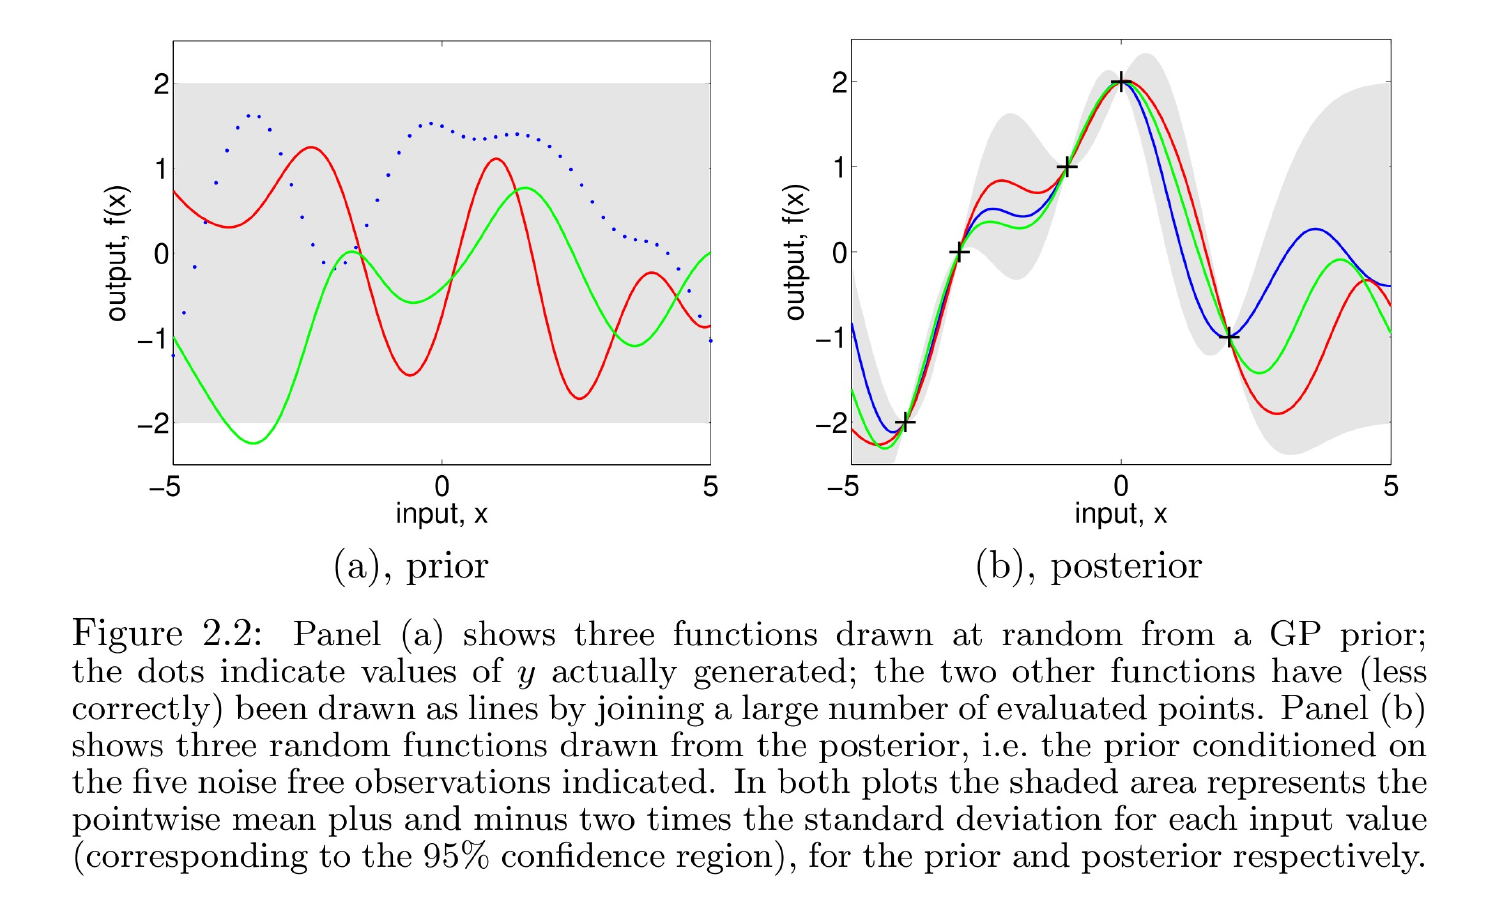
\includegraphics[width = \textwidth]{sampling.png}
\end{center}

\noindent To generate samples $\textbf{x} \sim \mathcal{N}(\textbf{m},K)$ with arbitrary mean $\textbf{m}$ and covariance generating multivariate matrix $K$ using a scalar Gaussian generator (which is readily available in many Gaussian samples
programming environments) we proceed as follows: first, compute the Cholesky
decomposition $L$ of the positive definite
symmetric covariance matrix $K = LL^{T}$, where $L$ is a lower triangular
matrix. Then generate $\textbf{u} \sim \mathcal{N}(\textbf{0}, I)$ by multiple separate calls
to the scalar Gaussian generator. Compute $\textbf{x} = \textbf{m} + L\textbf{u}$, which has the desired
distribution with mean $\textbf{m}$ and covariance $L\mathbb{E}[\textbf{uu}^{T}]L^{T} = LL^{T} = K$ (by the
independence of the elements of $\textbf{u}$).

\section{Problems}

\subsection{GP with RBF Kernel}
% Yash
Consider a Gaussian Process $f(x) \sim GP(0,K)$ where $K$ is the RBF kernel $K(x_1,x_2) = e^{\left( 
- \frac{(x_1 - x_2)^2}{2} \right)}$ where $x \in \R$ and mean is 0. We have one data point $D = \{ x_0 = 0, y_0 = -1 \}$. Answer the following:

\begin{enumerate}[label=(\alph*)]
    \item What is $-2\mu(x) + 4\sigma^2(x)$, where $\mu(x)$ and $\sigma(x)$ are mean and standard deviation of the posterior distribution $P(f(x)|D)$ when:
    \begin{itemize}
        \item $x = \sqrt{\log(4)}$
        \item $x \rightarrow \infty$
    \end{itemize}
    \item Let $y_1 = f(x = \sqrt{\log(4)})$ and $y_2 = f(x = -\sqrt{\log(4)})$ be 2 random variables. What is $\alpha + \beta$ where $\alpha$, $\beta$ = $\arg \max P(y_1,y_2|D)$ ?
\end{enumerate}

\noindent \textbf{Solution:} \\
% Annam

\noindent (a) We know \( P(f^*|\mathbf{x}^*,D) = \mathcal{N} \left( \mathbf{k}^T (K + \sigma^2 I)^{-1} \mathbf{y}, \mathcal{K}(\mathbf{x}^*, \mathbf{x}^*) - \mathbf{k}^T (K + \sigma^2 I)^{-1} \mathbf{k} \right). \) \\
Here as there is only one data point (\(x_0,y_0\))
\[ \mathbf{k}^T(K + \sigma^2 I)^{-1}\mathbf{y} = \frac{\mathcal{K}(\mathbf{x}^*, \mathbf{x}_0)\mathbf{y}_0}{(1 + \sigma^2 )} = \mu(x)  \]
\[\mathcal{K}(\mathbf{x}^*, \mathbf{x}^*) - \mathbf{k}^T (K + \sigma^2 I)^{-1} \mathbf{k} = 1-\frac{{\mathcal{K}(\mathbf{x}^*, \mathbf{x}_0)}^2}{(1 + \sigma^2 )} = \sigma^2(x)\]
Now using \( \mathbf{y}_0= -1\) \[-2\mu(x) + 4 \sigma^2(x) = 4 +\frac{\mathcal{K}(\mathbf{x}^*, \mathbf{x}_0)(2-4(\mathcal{K}(\mathbf{x}^*, \mathbf{x}_0))}{1+\sigma^2}  \]

\noindent For \(\mathbf{x}^*=\sqrt{\log(4)}\), we get \(\mathcal{K}(\mathbf{x}^*, \mathbf{x}_0)=\frac{1}{2} \) and for \(\mathbf{x}^*\rightarrow{} \infty \), we get \(\mathcal{K}(\mathbf{x}^*, \mathbf{x}_0)=0 \). \\
Putting the values back, we get \(-2\mu(x)+4\sigma^2(x)= \mathbf{4} \) for both cases. \\

% Sarthak
\noindent (b) Given the symmetry for positive and negative values of $x$, both $y_1$ and $y_2$ follow $\mathcal{N}(\mu = -1, \sigma^2 = 0.5)$. Hence the joint distribution will also be a Gaussian, and the position of maximum value will be the mean, which will be given as (using the formula mentioned in 1.4): \[ \mu = \frac{-1 \times 0.5 + -1 \times 0.5}{0.5 + 0.5} = -1 \]
Since the distribution has circular symmetry, $\alpha = \beta = -1$, giving us the answer $\mathbf{-2}$.

\subsection{Fitting GP on Data}
% Yash
Suppose we want to sample a point $\mathbf{x}$ such that a GP that is fit on $D$ exhibits the least variance there. Formulate the objective that gives us this. \\

\noindent \textbf{Solution:} \\
% Annam

\noindent We sample the point $\mathbf{x}$ which corresponds to minimum of the variance of the posterior distribution: \[ \arg \min_{x^*}  \left( \mathcal{K}(\mathbf{x}^*, \mathbf{x}^*) - \mathbf{k}^T (K + \sigma^2 I)^{-1} \mathbf{k} \right) \]
Qualitatively, it is very likely that this point will lie close to a dense cluster of the training data and hence exhibit lowest variance.

\subsection{1-D Regressor GP}
% Yash
We are estimating a 1-D regression function $f(x)$ as a Gaussian Process $GP(m(x),K(x,x'))$ where the kernel function $K(x,x') = \sigma_f^2 e^{\left( \frac{(x - x')^2}{2 \tau} \right)}$ and $m(x) = 0$. Each $y_i = f(x_i) + \epsilon_i$ where $\epsilon_i \sim \mathcal{N}(0,\sigma^2)$. Assume training data $D = \{ (\mathbf{x}_i,y_i \}_{i = 1}^N$. Express briefly in qualitative terms the shape of the mean of $f(x|D)$ posterior to seeing the training data $D$ in terms of the following properties:

\begin{enumerate}[label = (\alph*)]
    \item Noise $\sigma^2$ is very large
    \item Length scale $\tau$ changes from $10^{-4}$ to $10^4$
\end{enumerate}

\noindent \textbf{Solution:} \\
% Annam

\noindent (a) The posterior falls back to the prior since data is unreliable (very noisy). \\
\noindent Mathematically, we know \(P(\mathbf{f}|D) = \mathcal{N}(K(K + \sigma^2 I)^{-1} \mathbf{y}, \sigma^2 K(K + \sigma^2 I)^{-1})\). \\
Hence the mean = \((K(K + \sigma^2 I)^{-1} \mathbf{y}\) and variance = \(\sigma^2 K(K + \sigma^2 I)^{-1})\) \\
If noise is large then \(\sigma^2 I\) term dominates K hence mean \(=(K(K + \sigma^2 I)^{-1} \mathbf{y} \approx \frac{K\mathbf{y}}{\sigma^2} \approx \mathbf{0}\). \\
Using the same argument variance = \(\sigma^2 K(K + \sigma^2 I)^{-1}) \approx \frac{\sigma^2 K I}{\sigma^2} \approx K \). \\
So \(P(\mathbf{f}|D) \approx \mathcal{N}(\mathbf{0,K})\) which is equal to prior. \\

\noindent (b) As $\tau$ increases, because of kernel function having reduced flexibility (smaller range of values), the fluctuations will reduce, distribution becomes dense, and so the GP becomes very smooth.

%%%%%%%%%%% end of doc
\end{document}